\begin{enumerate}[label=\thesection.\arabic*.,ref=\thesection.\theenumi]
\numberwithin{equation}{enumi}

\item
consider a standard negative feedback transfer function configuration with
\begin{align}
G(s) = \frac{1}{(s+1)(s+2)}
\end{align}
and
\begin{align}
H(s) = \frac{s+\alpha}{s}
\end{align}
the closed loop system to have poles on the imaginary axis,the value of $\alpha$ should be equal to
%\centering
%\includegraphics[width=\columnwidth]{ee18btech11020.eps}
\begin{figure}[!ht]
\centering
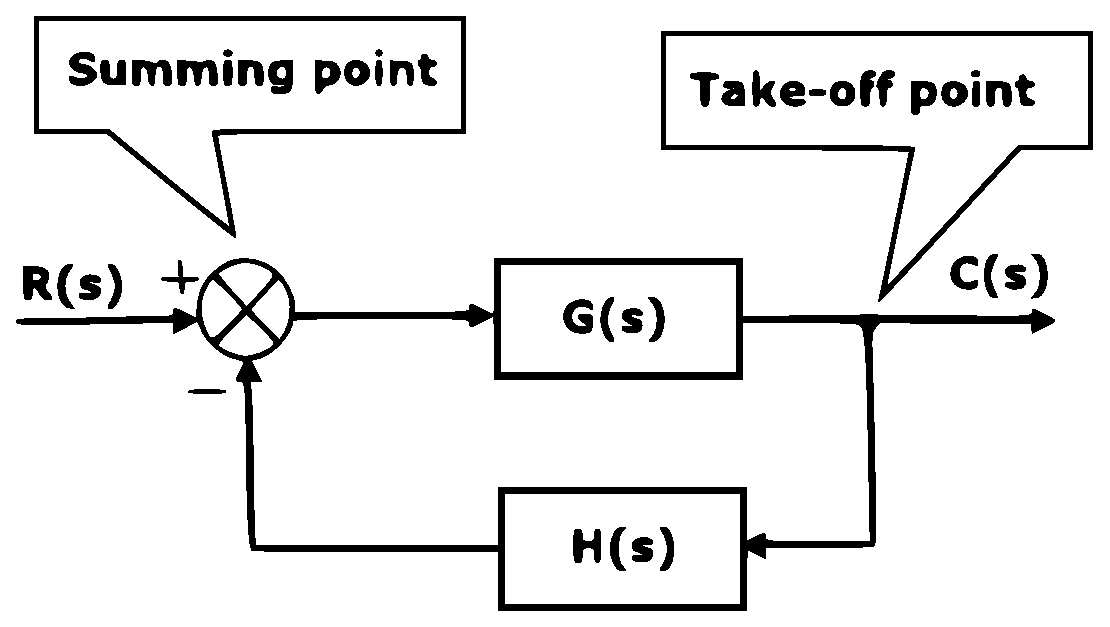
\includegraphics[width=\columnwidth]{./fig/ee18btech11020_basic_block_diagram.eps}
\caption{}
\label{fig:sec_order}
\end{figure}
\solution The transfer function for negative feedback is given by
\begin{align}
\frac{Y(s)}{X(s)} &= \frac{G(s)}{1+G(s)H(s)}
\end{align}
where 
\begin{align}
G(s) = \frac{1}{(s+1)(s+2)}
H(s) = \frac{s+\alpha}{s}
\end{align}
Characteristic equation is..,
\begin{align}
 1 + G(s)H(s) = 0
\\
=> 1 + \sbrak{\frac{1}{(s+1)(s+2)}}\sbrak{\frac{s+\alpha}{s}} = 0
\\
=> s^3+3s^2+3s+\alpha = 0
\end{align}
The Routh hurwitz criterion:-
This criterion is based on arranging the coefficients of characteristic equation into an array called Routh array.
For any characteristic equation q(s),
\begin{multline}
q(s) = a_0s^n+a_1s^{n-1}+.....+a_{n-1}s+a_n = 0
\end{multline}
Routh array can be constructed as follows..,
 
\myvec{s^n\\s^{n-1}\\s^{n-2} \\ \vdots}
 \myvec{a_0 & a_2 & a_4 & \cdots \\
a_1 & a_3 & a_5 & \cdots  \\
b_1 & b_2 & b_3 & \cdots \\
\vdots & \vdots & \vdots & \ddots &\vdots 
 \cdots \\}
 \\
 where
 \begin{align}
 b_1 =\frac{ a_1a_2-a_0a_3}{a_1}  
 \\
 b_2 =\frac{ a_1a_4-a_0a_5}{a_1} 
 \\
 c_1=\frac{ b_1a_3-a_1b_2}{b_1} 
\\
 c_2=\frac{ b_1a_5-a_1b_3}{b_1}  
\end{align}
For poles to lie on imaginary axis any one entire row of hurwitz matrix should be zero.
Constructing the routh array for the characteristic equation obtained in equation(\ref{eq:sec_order_op})
\begin{align}
 s^3+3s^2+3s+\alpha = 0
\end{align}
%
\begin{align}
\myvec{s^3\\s^2\\s^1 \\ s^0}
\myvec{1 & 3 \\ 3 & \alpha \\  \frac{9-\alpha}{3} & 0\\ \alpha & 0} \label{eq:sec_order_op_1}
\end{align}
For poles on j$\omega$ axis any one of the row should be zero.
\begin{align}
\frac{9-\alpha}{3} = 0 \hspace{5pt} or\hspace{5pt} \alpha = 0
\end{align}
But when $\alpha$ = 0 poles does not lie on the imaginary axis
\begin{align}
   9-\alpha = 0\\
   \alpha = 9
\end{align}
put $\alpha$ in the characteristic equation we get
\begin{align}
s^3+3s^2+3s+9=0
\end{align}
poles are 
\begin{align}
s = -3,-j\sqrt{3} ,j\sqrt{3}
\end{align}
\end{enumerate}